%%%%%%%%%%%%%%%%%%%%%%%%%%%%%%%%%%%%%%%%%%%%%%%%%%%%%%%%%%%%%%%%%%%%%%%%%%%%%
%% CipherScope -- submission to the Journal of Cryptographic Engineering.
%%
%% Ported from the ACM acmart (sigconf) source paper/manuscript-revised.tex
%% to the Springer Nature journal template, as recommended by the JCEN
%% submission guidelines:
%%   "Manuscripts should be submitted in LaTeX. We recommend using Springer
%%    Nature's LaTeX template and choosing the formatting option [iicol]."
%%
%% Class options:
%%   pdflatex  -- figures supplied as PDF (vector)
%%   sn-basic  -- Springer Nature basic reference style
%%   Numbered  -- numbered citations in square brackets, as JCEN requires
%%   iicol     -- two-column layout, as JCEN recommends
%%
%% Build:  tectonic -X compile manuscript.tex
%%         (or: pdflatex -> bibtex -> pdflatex -> pdflatex)
%%
%% Items still needing the authors' input are marked \todo{...} and render in
%% red. Search for "todo" before uploading; see SUBMISSION-CHECKLIST.md.
%%%%%%%%%%%%%%%%%%%%%%%%%%%%%%%%%%%%%%%%%%%%%%%%%%%%%%%%%%%%%%%%%%%%%%%%%%%%%
\documentclass[pdflatex,sn-basic,Numbered,iicol]{sn-jnl}

\usepackage{graphicx}
\usepackage{booktabs}
\usepackage{xcolor}
\usepackage{amsmath,amssymb}

% Long identifiers like GetCryptoContext() otherwise overflow the narrow
% column. Extra emergency stretch lets TeX loosen a line rather than let it
% run into the gutter; \code is \texttt with break opportunities at the
% word boundaries of a CamelCase identifier.
\setlength{\emergencystretch}{3em}
\newcommand{\code}[1]{\texttt{#1}}

% Marker for open items that the authors must supply before upload.
\newcommand{\todo}[1]{\textcolor{red!75!black}{[TODO: #1]}}

\begin{document}

\title[CipherScope: Observability and Diagnosis for OpenFHE]{CipherScope:
Runtime Semantic Observability and Diagnosis for OpenFHE Programs}

%% The corresponding author is marked with the starred \author* command.
%% TODO (optional): add \orgdiv{...} for each affiliation, and the 16-digit
%% ORCID of each author, if available.
\author*[1]{\fnm{Kimon Antonios} \sur{Provatas}}\email{kap4722@eid.utexas.edu}

\author[1]{\fnm{Ilias} \sur{Georgakopoulos-Soares}}

\author[1]{\fnm{Samuel-Karim Elyes} \sur{Benhamou}}

\affil*[1]{\orgname{The University of Texas at Austin}, \orgaddress{\city{Austin}, \state{Texas}, \country{USA}}}

\abstract{Applications built using fully homomorphic encryption (FHE) schemes
present several challenges for developers attempting to understand their
execution. Traditional profiling tools identify where execution time is spent,
but generally do not capture semantic properties relevant to the correctness
and efficiency of encrypted programs. Examples include whether multiple
rotations operate on the same ciphertext, whether generated evaluation keys
are subsequently used, and how much of the configured multiplicative-depth
budget is consumed during execution. Such properties are often best examined
at runtime. We present CipherScope, a diagnosis and observability system for
OpenFHE programs. CipherScope reconstructs program execution as a validated
graph of ciphertext versions, state transitions, and provenance information.
It applies a collection of conservative diagnostic rules to this graph to
identify potential optimizations and configuration problems. Each rule records
the evidence supporting its finding and provides an explanation when its
preconditions are not satisfied. An additional focus of the system is
measuring its observation boundary. Runs are assigned coverage
classifications, and only completely observed runs are included in the
evaluation. We evaluate CipherScope across CKKS, BFV, and BGV, measuring
tracing fidelity and workload coverage. We also verify that instrumentation
preserves program output for all three schemes. On a known-answer benchmark,
the system detects all seeded positive cases without triggering on the hard
negatives. On an independently authored workload corpus, six of eight
adjudicated findings were considered actionable. Applying the corresponding
changes produced speedups of up to 4$\times$.}

\keywords{Fully homomorphic encryption, OpenFHE, Runtime observability,
Dynamic program analysis, Performance diagnosis, Developer tools}

\maketitle

\section{Introduction}
\label{sec:intro}

An FHE program performs computations on encrypted data without requiring the
party performing the computation to access the underlying plaintext. This
property makes FHE useful in settings where sensitive data must be processed
by an untrusted or otherwise separate computing party. However, the
computational cost remains substantial. The performance of an implementation
can depend considerably on how the developer organizes operations, configures
the cryptographic context, and manages ciphertexts.

Understanding these choices is difficult with conventional profiling tools. A
profiler can identify expensive operations, but it generally cannot determine
whether those operations could have been reorganized or eliminated based on
their semantic properties.

Consider an OpenFHE program that packs a vector into one ciphertext, rotates
it by four indices, and adds the resulting ciphertexts. A line profiler will
identify the four \texttt{EvalRotate} calls as expensive operations. However,
it cannot determine whether all four calls operate on the same ciphertext
version. This distinction matters because rotations of the same ciphertext
can sometimes share an expensive precomputation. Whether this transformation
is valid also depends on the context's key-switching technique. Similarly, a
profiler cannot determine whether a rotation key generated during setup is
ever used during execution. These questions require information about
ciphertext identity, context configuration, and operation history.

CipherScope addresses this problem by observing calls made by an application
to OpenFHE~\cite{openfhe2022}. It does not instrument the internals of the
library. Instead, each observed call is associated with its source location
and the relevant input and output ciphertexts. Ciphertexts are represented
using versioned identities, so an operation that modifies a ciphertext in
place produces a new version rather than overwriting the previous one. The
recorded versions also carry scheme-dependent state, including level, scale,
slot count, and key-switching technique. Diagnostic rules operate on the
resulting execution graph. For example, a rotation-hoisting finding can
identify four rotations that read \texttt{ct\_0001:v0} under BV key
switching, along with the source lines on which the calls occurred and the
absence of a preceding compatible precomputation.

There are three main design considerations behind CipherScope. First, it
observes applications at runtime rather than relying on compiler
representations or library-level measurements. This allows it to capture
branches and parameters selected during execution. Second, the diagnostic
rules are conservative. They only produce findings when the required evidence
is available, and otherwise report why they cannot reach a conclusion.
Recommendations are expressed as experiments to try rather than predicted
speedups. Third, the system records the completeness of its observations.
Runs are classified as \texttt{COMPLETE}, \texttt{PARTIAL-PERMISSIVE}, or
\texttt{UNSUPPORTED}, and only \texttt{COMPLETE} runs are included in the
evaluation.

CipherScope has two frontends that produce a common trace representation. The
Python frontend wraps a live cryptographic context in a proxy. Its runner
intercepts the program's \texttt{GenCryptoContext} call, allowing existing
scripts to execute without modification. The C++ frontend uses a GCC plugin
to instrument the OpenFHE application boundary in a separate shadow build.
The original source tree and binary are left unchanged. Both frontends feed
the same validation, graph construction, twelve diagnostic rules, and
exporters. We also perform parity checks to verify that matching Python and
C++ programs produce equivalent traces.

This paper makes four contributions.

\begin{enumerate}
\item First, we introduce a source-attributed model of FHE execution that
  reconstructs ciphertext versions, state, rotation-key usage, and lineage
  from observed application calls (Sect.~\ref{sec:framework}). The observation
  boundary is measured explicitly. The model supports CKKS, BFV, and BGV,
  including differences in how multiplicative depth must be represented. In
  particular, CKKS and BGV expose a level progression, whereas BFV does not.
  Our measurements also show that BFV noise-scale degree is not cumulative
  and therefore cannot be used as a direct depth measurement
  (Sect.~\ref{sec:scheme}).
\item Second, we develop twelve conservative diagnostic rules over the
  reconstructed execution model (Sect.~\ref{sec:rules}).
\item Third, we describe an evaluation methodology for FHE observability
  tools (Sect.~\ref{sec:setup}). It includes coverage classifications,
  known-answer benchmarks with hard negatives, adjudication of real findings,
  before-and-after measurements for actionable recommendations, and
  deterministic regeneration of tables from raw experimental records.
\item Finally, we evaluate CipherScope on several workloads
  (Sect.~\ref{sec:results}). Six of eight adjudicated findings were actionable,
  and the corresponding changes were measured. We also retain and discuss
  both false positives rather than excluding them from the reported results.
\end{enumerate}

CipherScope is not intended to replace an FHE compiler, benchmark framework,
or conventional profiler. It also does not claim to be the first tool for
profiling FHE workloads. Sect.~\ref{sec:related} discusses related systems, while
Sect.~\ref{sec:limits} describes the limitations imposed by the observation
boundary and the supported operations.

\section{Background and Motivation}
\label{sec:background}

\subsection{FHE and the three schemes}

FHE allows computation to be performed directly on encrypted inputs. This
paper considers three schemes supported by OpenFHE: CKKS~\cite{ckks2017},
BFV~\cite{brakerski2012,fv2012}, and BGV~\cite{bgv2012}. CKKS supports
approximate arithmetic over encrypted real-valued vectors, while BFV and BGV
support exact arithmetic over packed integer vectors modulo a plaintext
modulus $t$.

Several properties of these schemes affect the diagnostics that CipherScope
can perform.

\paragraph{Multiplicative depth is an important resource.} A cryptographic
context is configured with a multiplicative depth, and
ciphertext--ciphertext multiplication consumes part of this budget. In CKKS
and BGV, this progression can be observed through ciphertext levels. Each
multiplication raises the level by one within a bootstrap epoch. BFV does not
expose an equivalent progression through \texttt{GetLevel()}, which returns
zero for every ciphertext. We discuss this distinction in
Sect.~\ref{sec:scheme}.

Depth exhaustion is not always reported as an explicit runtime error. In BGV,
for example, a computation can produce a ciphertext that subsequently
decrypts to an incorrect value. Consequently, depth analysis is relevant to
correctness as well as performance.

\paragraph{Rotations introduce another source of overhead.} A rotation by
index $i$ generally requires a corresponding rotation key to have been
generated during setup. Keys that are never used increase setup time and
memory consumption. Multiple rotations of the same ciphertext version can
also share a precomputation through \texttt{EvalFastRotationPrecompute}, but
this is only valid under particular conditions. The input ciphertexts must be
identical, and the key-switching technique must support the transformation.

\paragraph{The schemes also differ in their treatment of precision.} CKKS is
approximate, and accumulated numerical error is an important consideration.
BFV and BGV are exact schemes; incorrect decrypted output indicates a
correctness failure rather than ordinary approximation error. This
distinction affects which diagnostic rules are meaningful and when they
should abstain.

\subsection{OpenFHE and the application boundary}

OpenFHE~\cite{openfhe2022} is an open-source C++ library for FHE that also
provides a Python wrapper. A typical application creates a cryptographic
context from a set of parameters, generates keys, and invokes operations such
as \texttt{Encrypt}, \texttt{EvalAdd}, \texttt{EvalMult},
\texttt{EvalRotate}, \texttt{EvalBootstrap}, and \texttt{Decrypt}.

CipherScope uses this interface as its observation boundary. It records calls
that cross the application-facing OpenFHE interface but does not inspect the
internal implementation of those calls. Number-theoretic transforms,
key-switching internals, and memory-management operations are outside its
scope.

This distinction is relevant when comparing CipherScope with tools that
profile the library itself. Such tools can characterize lower-level execution
costs, whereas CipherScope focuses on the choices made by an application. The
two types of information are complementary.

\subsection{A motivating example}
\label{sec:example}

OpenFHE includes \texttt{simple-integers.py}, a 103-line BFV example that
encrypts three integer vectors, performs additions and multiplications, and
rotates the first ciphertext by 1, 2, $-1$, and $-2$. We use this program as
a running example because it was developed independently of CipherScope and
exercises several of the properties considered by our analysis.

Figure~\ref{fig:overview} compares a conventional timing profile with the
trace produced by CipherScope.

\begin{figure*}
  \centering
  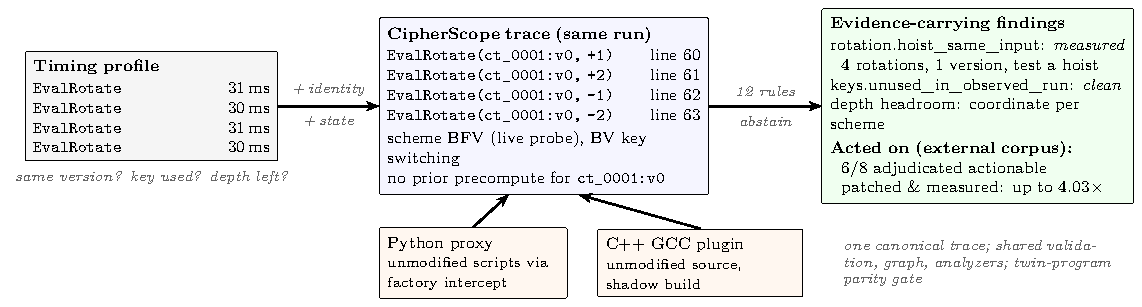
\includegraphics[width=0.92\textwidth]{Fig1}
  \caption{What a timing profile keeps versus what CipherScope records for
  the same four-rotation BFV run (the upstream \texttt{simple-integers.py}
  example of Sect.~\ref{sec:example}), and where the added facts go: a validated
  version/state graph, twelve conservative rules, and---on an independently
  authored corpus---adjudicated findings whose patches were measured. Both
  frontends emit one canonical trace.}
  \label{fig:overview}
\end{figure*}

The timing profile shows that the four \texttt{EvalRotate} calls account for
a significant portion of execution time. It does not provide enough
information to determine whether the rotations can share a precomputation.
CipherScope identifies that all four operations read \texttt{ct\_0001:v0},
with rotation indices $\{-2,-1,1,2\}$. The context uses BV key switching, and
no compatible \texttt{EvalFastRotationPrecompute} call occurs before the
group.

These observations satisfy the preconditions of the rotation-hoisting rule.
The finding identifies the four events and suggests testing a shared
precomputation. This recommendation is permitted under BV because a separate
gate check (Sect.~\ref{sec:rq1}) verified that the shared precomputation produces
the same result as regular rotations under this technique.

The same trace also provides information about the multiplication chain and
rotation-key usage. In this example, every generated rotation key is used, so
the unused-key rule does not report a finding. Both the original BFV program
and a BGV counterpart were traced completely (\texttt{COMPLETE}). Each
produced 17 semantic calls, and the decrypted outputs were bit-identical to
the corresponding uninstrumented executions (Sect.~\ref{sec:rq2}).

\section{Threat Model and Scope}
\label{sec:threat}

CipherScope is intended as a development-time diagnostic tool. Its security
assumptions are limited to the environment in which a developer runs their
own application.

We assume that the developer is tracing a program they are authorized to
inspect, using data they are permitted to access. There is no adversary in
the threat model. The problems targeted by CipherScope are implementation and
configuration issues, including unnecessary operations, unused evaluation
keys, excessive depth, and testing-only settings that remain enabled in
production-oriented code.

Traces can contain sensitive information. They include argument and result
representations, exception messages, and absolute source paths. In shadow
mode, when a developer supplies a secret key, traces can also contain
decrypted values used for precision comparisons. CipherScope does not record
secret-key material or ciphertext coefficients. Nevertheless, traces should
be treated as confidential development artifacts. We do not claim that they
are free of information leakage.

The system makes no cryptographic security claim. One configuration rule
checks whether a declared context uses \texttt{HEStd\_NotSet} and identifies
this as a testing-only configuration. This is a configuration observation,
not a security analysis. CipherScope does not estimate bit security or
determine whether a parameter set is secure. Side-channel attacks, fault
attacks, and the implementation security of OpenFHE
itself~\cite{safetycentric2025} are outside the scope of this work.

The observation boundary also requires cooperation from the application. The
Python frontend only observes calls that pass through its proxy, while the
C++ frontend records calls instrumented by its plugin. Applications can
bypass these mechanisms. Sect.~\ref{sec:coverage} describes how the system
identifies several known bypass patterns and assigns incomplete coverage
classifications when necessary.

\section{The CipherScope Framework}
\label{sec:framework}

\subsection{Design principles}
\label{sec:principles}

CipherScope follows four design principles.

\paragraph{Observe execution where application decisions are made.}
Developers choose which ciphertexts to operate on, which keys to generate,
and how to configure the cryptographic context. These decisions are visible
at the application boundary. Instrumenting lower-level library operations
would provide additional information about implementation costs, but it would
not directly capture the semantic relationships between application-level
operations. Conversely, static analysis alone cannot always determine which
branch or parameter configuration was used during a particular execution.

\paragraph{Represent ciphertexts using explicit identities.} Determining
whether two rotations operate on the same ciphertext requires a stable
representation of ciphertext identity. CipherScope treats ciphertext versions
as immutable graph nodes. An operation that modifies a ciphertext in place
creates a new version, preserving the previous state for subsequent analysis.
This representation allows the system to distinguish multiple operations on
the same version from operations on values that were modified between calls.

\paragraph{Separate collection from analysis through a shared trace format.}
The Python proxy and GCC plugin have different implementations, but both
produce documents conforming to the same schema. Validation, graph
construction, diagnostics, and export are performed by a common pipeline.
Findings can therefore be inspected independently of the frontend that
produced them.

\paragraph{Abstain when required evidence is unavailable.} A finding must be
supported by recorded events or an explicit developer assertion. If the
system cannot establish a required condition, it reports the missing
information rather than treating the absence of evidence as evidence that no
problem exists. Recommendations are expressed as experiments. The system
reports the combined execution time of the operations involved, which we call
the stake, but does not estimate the speedup of a proposed transformation.

\subsection{The trace and ciphertext versions}
\label{sec:trace}

Each execution produces a validated bundle containing a schema-versioned
trace, a derived ciphertext graph, diagnostic findings, and several export
formats. The trace records events, ciphertext versions, context information,
and coverage metadata. Exporters support CSV, Perfetto, and a static HTML
report.

Events contain the canonical operation name, source location, wall-clock and
CPU duration for the complete call, input and output ciphertext versions,
relevant state, semantic arguments, and execution status. Failed calls are
represented as error events rather than omitted from the trace.

Ciphertext identity is based on versions. A result may receive an identifier
such as \texttt{ct\_0002:v0}. In-place operations, including
\texttt{EvalAddInPlace} and \texttt{RescaleInPlace}, create a subsequent
version of the operand. Later operations refer to that version. Copies,
moves, and container storage preserve identity, while destruction of an
object does not allow its identifier to be reassigned to a later object at
the same memory address. These behaviors are checked against the actual
library through integration gate tests.

Recording has explicit resource limits. Events and finalized ciphertext
states are written to disk during execution. Maximum event-count and
trace-size limits prevent unbounded recording; when a limit is reached, the
trace is marked as truncated without stopping the underlying workload.
Finalization and analysis are not streamed. Materializing the resulting graph
currently requires approximately 2.2\,KB of trace data and 30\,KB of peak
memory per event (Sect.~\ref{sec:rq5}).

\subsection{Two frontends, one trace}
\label{sec:frontends}

The \textbf{Python frontend} wraps a native cryptographic context in a proxy
object. Calls passing through the proxy are recorded. In strict mode, an
operation that the compatibility registry cannot classify is rejected.
Permissive mode forwards the call but marks the resulting trace as
incomplete.

The runner supports existing Python scripts by intercepting their
\texttt{GenCryptoContext} call and attaching the returned context to the
proxy. This allows the corpus programs to run without source modifications.
Programs that obtain their context through another mechanism must attach it
manually.

The \textbf{C++ frontend} is implemented as a GCC plugin. The command
\texttt{cipherscope profile <binary>} locates the target's CMake build and
creates an instrumented \emph{shadow} build. The original source tree and
binary are not modified. The plugin instruments application-boundary OpenFHE
call sites during compilation.

Instrumentation occurs before optimization. We verify that the resulting
events and source locations remain consistent across \texttt{-O0},
\texttt{-O2}, and \texttt{-O3}. Operator overloads such as $*$, $+$, $+{=}$,
and unary $-$ are normalized to the same event representation as the
corresponding named operations. Concurrent OpenMP calls are recorded
individually.

The resulting native trace is converted to the same schema used by the Python
frontend. All subsequent processing is shared. We also compare eight pairs of
Python and C++ programs implementing equivalent computations. Their traces are
equivalent across the operations covered by the parity tests.

\subsection{Coverage classification}
\label{sec:coverage}

Since neither frontend can observe calls that bypass its instrumentation
boundary, each execution receives a coverage classification.

A run is classified as \texttt{COMPLETE} when it uses strict mode, finishes
successfully, contains at least one traced call, forwards no untraced
operations, and contains no detected bypass pattern. A preflight syntax-tree
scan checks for raw-context access, module-level \texttt{Eval*} free
functions, and \texttt{GetCryptoContext()} escapes.

\texttt{PARTIAL-PERMISSIVE} and \texttt{UNSUPPORTED} runs are excluded from
all evaluation populations that require complete observation. This
classification is an operational measure rather than a formal guarantee. In
particular, the preflight scan cannot detect every possible way of bypassing
the instrumentation.

The rejected operations are also useful information. When we traced five
upstream OpenFHE integer-scheme examples (Sect.~\ref{sec:rq2}), three were
rejected in strict mode. The coverage record identified
\texttt{MultipartyKeyGen} and \texttt{ReKeyGen}, which belong to
threshold-FHE and proxy-re-encryption workflows not currently covered by the
operation manifest. These operations are reported explicitly rather than
forwarded without observation.

\subsection{A scheme-parametric state model}
\label{sec:scheme}

CipherScope records the scheme associated with each trace and interprets
ciphertext state accordingly. Several measurements on the pinned OpenFHE
build influenced the state model.

The Python wrapper does not provide a scheme getter. When declared parameters
are available, those parameters are used. Otherwise, CipherScope identifies
CKKS by calling \texttt{GetModulusCKKS()}, which succeeds for CKKS and raises
an exception for the integer schemes. BFV and BGV are then distinguished
using their scaling techniques: BFV uses \texttt{NORESCALE}, whereas BGV does
not. The trace records the evidence used to identify the scheme. Gate checks
verify this behavior for all three schemes and the supported scaling
techniques.

BFV requires separate treatment of multiplicative depth. Its
\texttt{GetLevel()} method returns zero for every ciphertext. We initially
considered using noise-scale degree as an alternative, since it begins at one
and increases following multiplication. However, measurements showed that the
value is not cumulative across arbitrary computation paths. On the pinned
build, adding a degree-1 ciphertext to a degree-2 ciphertext produces a
degree-1 result. This loses information about the multiplication history of
one operand.

Our initial implementation used noise-scale degree to estimate BFV depth. It
passed the seeded benchmark because those test cases contained pure
multiplication chains. It failed on a C++ twin program whose final addition
combined ciphertexts with different depths. We therefore changed the model to
count recorded ciphertext--ciphertext multiplications along the deepest
lineage. BFV depth findings are consequently marked as inferred rather than
measured. Each finding identifies its coordinate as either
\texttt{ciphertext\_levels} or \texttt{recorded\_multiplications}.

The configured BFV depth also requires careful interpretation. It is related
to the available noise budget, but it is not a direct counter of the number
of multiplications that can be performed. In our measurements, a depth-2 BFV
context correctly executed three consecutive multiplications. Depth-2 and
depth-3 contexts also exhibited the same capacity for the operands tested.
Since capacity depends on the values involved, a computation can exceed its
effective budget and decrypt incorrectly without raising a runtime exception.
The depth-headroom rule therefore reports an estimate based on the observed
inputs rather than a direct measurement of remaining capacity.

CKKS and BGV expose a more consistent level progression. In both schemes,
multiplication advances the level by one. This behavior held across the four
scaling techniques tested. Packing also differs between the schemes: the
integer schemes support $N$ slots, while CKKS supports $N/2$.

Bootstrapping is not supported for BFV or BGV on the pinned build. Calls to
\texttt{EvalBootstrapSetup} raise a ``Not supported'' exception. The
bootstrap-related rule uses this information to abstain on these schemes.

\subsection{Diagnosis rules}
\label{sec:rules}

CipherScope currently implements twelve diagnostic rules. Each rule specifies
its preconditions, supporting evidence, diagnosis, and suggested experiment.
When the required information is unavailable, it records the reason for
abstaining.

\paragraph{Repeated compatible rotations.} This rule identifies two or more
\texttt{EvalRotate} calls with different indices that read the same
ciphertext version. The calls must have matching context, key tag, scaling
state, and key-switching technique. The technique must also have passed gate
checks establishing equivalence between regular rotations and the proposed
shared precomputation. Currently, this evidence exists for HYBRID and BV. The
rule additionally requires that no compatible precomputation occurred earlier
and that no in-place mutation intervened.

When these conditions hold, CipherScope suggests testing
\texttt{EvalFastRotationPrecompute}. It reports the combined execution time of
the rotations as the stake. It does not claim that this time will be saved.
Missing metadata or an unsupported technique causes the rule to abstain.

\paragraph{Rotation keys unused in the observed run.} This rule compares the
rotation indices requested during key generation with the indices used by
\texttt{EvalRotate} calls. Keys not used in the observed execution are
reported. The finding is limited to the current run: an unused key may still
be required for another input or execution path.

\paragraph{Observed depth headroom.} This rule compares configured depth with
the executed depth, using the appropriate scheme-dependent coordinate from
Sect.~\ref{sec:scheme}. It also reserves one level when the deepest ciphertext
has a deferred rescale. This adjustment was introduced after an adjudicated
false positive showed that the recorded level could precede a committed level
by one operation (Sect.~\ref{sec:rq3b}).

The rule abstains when the depth model cannot be fully resolved. For example,
opaque calls such as \texttt{EvalChebyshevSeries} and
\texttt{EvalLogistic} may hide part of a computation's depth progression. Its
reported headroom is an upper bound when internal library operations are not
visible.

\paragraph{Testing-only security configuration.} This rule identifies
declared uses of \texttt{HEStd\_NotSet}. It only applies when the run
declares its parameters, since the security level cannot be read from a live
context. Runs without declared parameters are not classified by this rule.

The remaining rules use similar precondition checks. Bootstrap restoration
identifies cases where a bootstrap restores more levels than the subsequent
computation uses. It requires an input deeper than the fixed level to which
bootstrap outputs return, and it abstains on BFV and BGV because
bootstrapping is unsupported on the pinned build.

Packing utilization, public-value provenance, and repeated public encodings
require explicit developer annotations. CipherScope does not infer semantic
plaintext content from encrypted ciphertexts. Serial reduction review is
limited to regions annotated by the developer as associative.

Two precision rules require shadow mode, a secret key, and developer-provided
checkpoints. They only apply to CKKS. Checkpoint differences smaller than 3.0
absolute bits are ignored because CKKS decryption uses noise flooding. We
measured a standard deviation of 0.68 bits for this variation; an earlier
threshold of 1.0 bit produced a false-positive rate close to ${\sim}5\%$ on
noise alone. The precision rules abstain on the exact schemes.

Finally, the depth-critical-path rule is informational. It reports the
multiplication lineage when available but does not contribute to the
precision evaluation in Sect.~\ref{sec:rq3b}.

\section{Experimental Setup}
\label{sec:setup}

We organize the evaluation around six research questions.

\paragraph{RQ1:} Does tracing preserve program behavior and reconstruct state
correctly across the three schemes?

\paragraph{RQ2:} What fraction of real workloads can be completely observed?

\paragraph{RQ3:} What is the recall on known-answer programs, and what
precision is achieved on real findings?

\paragraph{RQ4:} Do validated findings result in measurable improvements?

\paragraph{RQ5:} What is the overhead of tracing?

\paragraph{RQ6:} Can the system identify misconfigurations in real programs?

\medskip
\noindent All experiments use OpenFHE~1.5.1 and Python wrapper 1.5.1.0, pinned
to a specific commit. We define an \emph{evidence lane} as an exact
combination of operating system, toolchain, and build configuration on which
the integration gate has been executed.

The authoritative lane is an Ubuntu 24.04 x86\_64 container using GCC 13.3,
built and executed on a TACC Lonestar6 node. Additional lanes include a
bare-metal Rocky Linux 8.10 build with GCC 15.2, a macOS arm64 developer
build, and an x86\_64 Docker environment running under emulation. Each lane
archives a feasibility artifact containing native-module hashes. These hashes
allow individual run bundles to be associated with the build used to produce
them.

We evaluate four groups of programs.

The first is a \emph{seeded benchmark} consisting of 61 known-answer cases
(28 CKKS, 17 BFV, 16 BGV). Each rule has positive cases that should trigger
findings and hard negatives that should not. Expected values can be derived
manually from the corresponding source programs.

The second is a \emph{CKKS corpus} containing 16 gallery examples and four
workloads from an independently authored regression suite, pinned by commit.

The third is an \emph{integer-scheme corpus} consisting of five BFV and BGV
examples distributed with the pinned wrapper.

The fourth is a \emph{designed impact suite}. It pairs prescriptive rules with
minimal programs, patches that follow the corresponding recommendations, and
subsequent re-traces.

For the real-finding precision evaluation, we exported every finding from
every completely observed CKKS corpus run. Two AI reviewers performed the
adjudication rather than human reviewers. The first reviewer completed an
initial pass. The second performed a blind review without access to the first
reviewer's verdicts and could run depth-reduction experiments on a scratch
copy of the corpus. Disagreements were resolved in favor of the reviewer who
performed the experiment. This procedure is a limitation of the evaluation.
The rubric, verdicts, and experiment transcripts are included in the artifact
so that the findings can be reviewed independently.

Tables and figures are regenerated from checksummed raw records using
deterministic generators. Regeneration produces byte-identical output, which
is verified by an automated test. The figures are generated from the
resulting tables rather than manually entered values.

Table~\ref{tab:summary} summarizes the main results.

\section{Results and Discussion}
\label{sec:results}

Table~\ref{tab:summary} reports the main evaluation results. The following
sections discuss each research question, including cases where the results
are limited by the current implementation.

\begin{table*}
  \caption{Headline results and evaluation populations. Each row is
  regenerated from checksummed raw records. Evidence lanes are defined in
  Sect.~\ref{sec:setup}.}
  \label{tab:summary}
  \small
  \begin{tabular}{@{}llr@{}}
    \toprule
    \textbf{Question} & \textbf{Population} & \textbf{Result} \\
    \midrule
    \multicolumn{3}{@{}l}{\emph{RQ1 Fidelity} (Sect.~\ref{sec:rq1})} \\
    \quad CKKS output deviation   & authoritative lane      & $2.2\times10^{-13}$ \\
    \quad BFV/BGV output          & seeded + C++ gate       & bit-identical \\
    \quad Integration gate        & 4 evidence lanes        & 40--42 checks \\
    \quad Cross-lane parity       & platform-independent    & 0 disagreements \\
    \quad C++/Python twin parity  & 8 twin programs         & equivalent \\
    \midrule
    \multicolumn{3}{@{}l}{\emph{RQ2 Coverage} (Sect.~\ref{sec:rq2})} \\
    \quad CKKS corpus             & 20 workloads, strict    & 20/20 \\
    \quad Integer-scheme corpus   & 5 workloads, strict     & 2/5 \\
    \quad C++ upstream examples   & 6 programs              & 6/6 \\
    \midrule
    \multicolumn{3}{@{}l}{\emph{RQ3 Finding quality} (Sect.~\ref{sec:rq3}, \ref{sec:rq3b})} \\
    \quad Seeded recall           & 31 positives, 12 rules  & 31/31 \\
    \quad Seeded false positives  & 44 hard negatives       & 0 \\
    \quad Adjudicated precision   & 8 in-scope findings     & 6/8 \\
    \midrule
    \multicolumn{3}{@{}l}{\emph{RQ4 Impact} (Sect.~\ref{sec:rq4})} \\
    \quad Performance findings    & 3 patches, measured     & 1.09--4.03$\times$ \\
    \quad Security findings       & 3 patches, measured     & see Fig.~\ref{fig:impact} \\
    \quad Designed rule pairs     & 10 before/after pairs   & 10/10 \\
    \midrule
    \multicolumn{3}{@{}l}{\emph{RQ5 Cost} (Sect.~\ref{sec:rq5})} \\
    \quad Absolute overhead       & 12 workloads, 3 reps    & 0.4--2.3\,s \\
    \quad Relative, $\geq$100\,s  & 2 workloads             & 0.7--1.8\% \\
    \quad Trace size              & $10^2$--$10^5$ events   & 2.2\,KB/event \\
    \midrule
    \multicolumn{3}{@{}l}{\emph{RQ6 Misconfiguration} (Sect.~\ref{sec:rq6})} \\
    \quad Declared \texttt{HEStd\_NotSet} & 10 real programs & 5 true positives \\
    \bottomrule
  \end{tabular}
\end{table*}

\subsection{RQ1: Tracing fidelity}
\label{sec:rq1}

Tracing fidelity is a prerequisite for the other results. If instrumentation
changes program behavior, then findings based on the resulting trace may not
describe the original application.

We evaluate fidelity by running each gate program with and without
instrumentation and comparing decrypted outputs. For CKKS, we compare the
numerical results using a tolerance. The observed deviation is four orders of
magnitude below that tolerance. For BFV and BGV, output comparison is exact:
instrumented runs reproduce the direct execution results bit for bit.

The C++ integration gate uses the same general approach, comparing the
printed output of instrumented and uninstrumented binaries. We also run the
gate across four evidence lanes to check for platform-dependent behavior.

All platform-independent checks agree. There are two qualifications. One
check reads \texttt{/proc} and is skipped on macOS. In addition, two checks
were introduced after the two cluster archives had been generated, so only
the emulated lane has executed the complete set. The emulated lane uses a
different binary and native-module hash and is not treated as authoritative.
We report the cluster results separately rather than combining these
measurements.

We also evaluate whether the two frontends produce equivalent traces. Eight
twin programs cover rotations, in-place operators, aliasing, exceptions,
vector composites, BFV, BGV, and checkpoints. The traces produced by the
Python and C++ frontends are equivalent for these programs. This supports the
use of a shared trace representation, although the parity evaluation is
limited to the tested cases.

\subsection{RQ2: Coverage of real workloads}
\label{sec:rq2}

Coverage determines which executions can be included in the diagnostic
evaluation. We therefore report the fraction of workloads classified as
\texttt{COMPLETE} rather than the number of programs that successfully
execute.

All 20 CKKS workloads are completely observed in strict mode. This required
adding support for three operations used by the corpus:
\texttt{EvalLogistic}, \texttt{EvalSumRows}, and \texttt{EvalSumCols}. Before
these additions, three of the four independently authored workloads were
classified as partially observed. The coverage classification prevented their
inclusion in the complete-run population.

The integer-scheme corpus provides a less favorable result. Only two of five
workloads are completely observed. Both produce rotation-hoisting findings on
programs that were not written by the CipherScope authors. The other three are
rejected because they use threshold FHE through \texttt{MultipartyKeyGen} or
proxy re-encryption through \texttt{ReKeyGen}, neither of which is covered by
the current operation manifest.

The corpus also exposed three read-only context getters missing from the
non-semantic allowlist. These had independently caused three workloads to be
rejected. We added the missing operations, but the final coverage figure
remains 2/5. This result reflects the current supported operation set rather
than the ability to execute the programs themselves.

\subsection{RQ3: Recall on known-answer programs}
\label{sec:rq3}

Recall cannot be measured directly on arbitrary real programs because the
expected findings are not known in advance. The seeded benchmark provides a
controlled evaluation population with expected positives, hard negatives, and
cases where the correct behavior is to abstain.

The benchmark includes cases such as a declared precision tolerance applied to
an exact scheme. In this situation, the precision rule should not report a
measurement because the relevant analysis is not supported.

All seeded positive cases are detected, and none of the hard negatives
produces a finding (Table~\ref{tab:summary}). These results establish recall
on the constructed benchmark, not on arbitrary real workloads.

The benchmark also exposed a limitation in our initial BFV depth model. As
described in Sect.~\ref{sec:scheme}, the original implementation passed the
seeded tests because they contained pure multiplication chains. A C++ twin
program with a final addition between ciphertexts of different depths exposed
the problem. We corrected the model and added a regression case to cover this
execution pattern. This example illustrates that the known-answer benchmark
is sensitive to the range of computation structures represented in its test
cases.

Figure~\ref{fig:ablation} presents a semantic ablation of the trace. We
re-analyze the same executions using three progressively richer
representations to determine which information each rule requires. One rule
can operate using timings and source locations alone. Five additional rules
require per-call state. The remaining six, including rotation hoisting,
provenance, packing, and serial reduction, require ciphertext-version
identity. This analysis helps quantify the contribution of the trace model,
although it is an ablation of CipherScope's own representation rather than a
comparison with an external profiler.

\begin{figure}
  \centering
  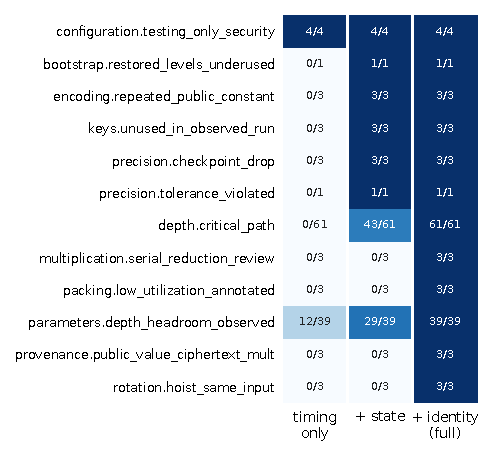
\includegraphics[width=\linewidth]{Fig2}
  \caption{Which part of the trace each rule needs. The same seeded runs are
  re-analyzed under three progressively richer views; cells show positives
  recovered out of positives available. One rule survives on timings alone;
  six require ciphertext version identity. This is an ablation of
  CipherScope's own trace, not a run of an external profiler.}
  \label{fig:ablation}
\end{figure}

\subsection{RQ3: Precision on real findings}
\label{sec:rq3b}

The CKKS corpus produced twelve findings. Four were depth-critical-path
reports. Since this rule is informational and reports whenever lineage
exists, these findings are excluded from the precision denominator.

The remaining eight findings consist of six actionable true positives and two
false positives.

The first false positive resulted from an observation limitation. The
depth-headroom rule reported available headroom, but both attempted depth
reductions failed inside a two-iteration \texttt{EvalBootstrap}. The internal
level consumption of this operation is not exposed through the ciphertext
state available to CipherScope.

The second false positive was caused by an implementation defect. The rule
reported headroom that did not exist because the final ciphertext had a
deferred rescale. Its recorded level did not yet reflect the additional
committed level. We modified the depth rule to reserve a level when a pending
rescale is present. The current rule therefore avoids this particular error.

We retain the original adjudicated verdict in the reported precision.
Replacing it with the result of the corrected implementation would make the
table inconsistent with the archived evaluation records. The resulting 6/8
precision figure is consequently lower than the current rule's performance on
that particular case would suggest.

\begin{figure}
  \centering
  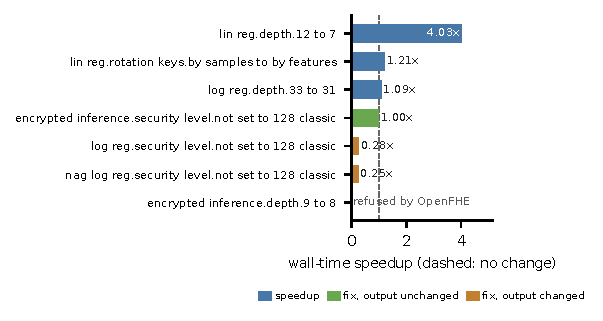
\includegraphics[width=\linewidth]{Fig3}
  \caption{Measured outcome of every attempted transformation on the
  external corpus. Enabling standard security enforcement was free on the
  inference workload but cost 3.5--4$\times$ on the two training workloads
  \emph{and changed their numerical results}, because enforcement enlarges
  the ring: the finding is actionable either way, and the trade is the
  developer's. The patch for the adjudicated false positive was refused by
  OpenFHE and is retained as evidence.}
  \label{fig:impact}
\end{figure}

\subsection{RQ4: Impact of acting on findings}
\label{sec:rq4}

We evaluate the practical value of findings by applying the recommended
changes and measuring the resulting programs. Each patch is checked using the
workload's existing correctness test. Figure~\ref{fig:impact} summarizes the
results.

The three performance findings produced measurable improvements. The largest
improvement came from reducing a configured depth of 12 to the observed value
of 7. This change produced a speedup of approximately 4$\times$.

The security-related findings had different effects. Enabling standard
128-bit security enforcement was free for one workload because its parameters
already satisfied the required ring size. For the two training workloads,
however, the larger ring increased execution time by approximately
3.5--4$\times$ and changed the numerical results. These results show that
security configuration can introduce a substantial performance and accuracy
trade-off. CipherScope reports the configuration issue, but the appropriate
choice depends on the application's requirements.

One patch corresponding to an adjudicated false positive was rejected by
OpenFHE at runtime. We retain this result in the figure rather than removing
it from the impact evaluation.

The designed impact suite evaluates whether each prescriptive rule behaves as
expected in a controlled setting. Each rule is paired with a minimal program,
a patch following the recommendation, and a subsequent re-trace. All ten
pairs behave as designed. One case is particularly relevant: correcting a
testing-only security configuration makes the toy program approximately four
times slower. This result is included to show that resolving a diagnostic
finding does not necessarily improve performance.

\begin{figure*}
  \centering
  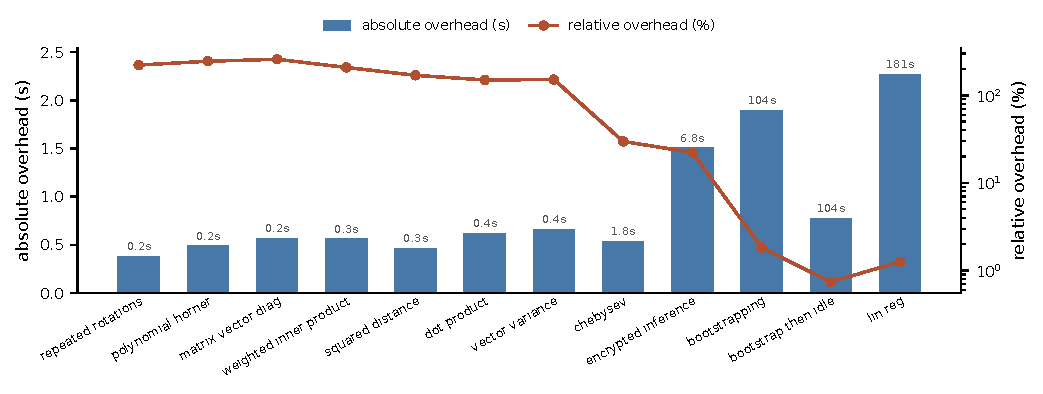
\includegraphics[width=0.92\textwidth]{Fig4}
  \caption{Per-workload tracing cost, sorted by baseline duration. Bars:
  absolute overhead (recording, finalization, and analysis). Line (log
  scale): the same cost relative to the baseline. The absolute cost is
  roughly fixed, so the relative cost falls from a few multiples on
  sub-second examples to under 2\% on workloads of 100\,s or more. Three
  matched repetitions per workload, one machine.}
  \label{fig:overhead}
\end{figure*}

\subsection{RQ5: Cost of tracing}
\label{sec:rq5}

The overhead measurements show that tracing introduces a relatively small
absolute cost for most workloads. The cost is dominated by recording,
finalization, and analysis rather than by the individual instrumented calls.

Figure~\ref{fig:overhead} reports absolute and relative overhead. Absolute
overhead remains approximately constant across a twelve-workload corpus
spanning three orders of magnitude in execution time. Relative overhead is
therefore higher for short examples and decreases for longer workloads. For
workloads taking at least 100\,s, the measured relative overhead ranges from
0.7\% to 1.8\%. CPU overhead on the longer workloads is within measurement
noise of zero.

We also perform an event-count sweep from $10^2$ to $10^5$ events. Run-phase
overhead remains bounded, while trace size grows approximately linearly at
2.2\,KB per event. Finalization is the main scalability limitation because it
materializes the trace rather than processing it incrementally.

At $10^5$ events, materialization and analysis peak at approximately
3.2\,GB of resident memory. The deep-bootstrap seeded case requires
substantially more memory, peaking near 7\,GB. On a memory-capped machine,
the process is killed below roughly 8\,GB, resulting in a missing bundle
rather than a recorded error. This behavior is documented in the artifact.

The event-count measurements are single runs on shared machines. They are
useful for identifying the scaling behavior of the current implementation,
but should not be interpreted as stable performance estimates.

\subsection{RQ6: Misconfiguration in real programs}
\label{sec:rq6}

We evaluate the configuration rule on ten real programs. Five declare
\texttt{HEStd\_NotSet}, which the rule identifies as a testing-only setting.
Three findings occur in the external suite. All three were considered
actionable and were corrected and measured as part of RQ4.

The remaining two occur in upstream OpenFHE examples, where the setting is
intentionally used to keep the examples computationally tractable. Both were
adjudicated as non-actionable. The other five programs have no such
configuration, and the rule produces no false positives.

The precision rules abstain on all ten programs because the unmodified
applications do not declare checkpoints. This prevents CipherScope from
measuring numerical precision changes on these workloads. It is a limitation
of the current annotation-based approach, but it also avoids reporting
measurements that were not actually performed.

\section{Limitations}
\label{sec:limits}

\paragraph{The observation boundary.} The primary limitation is the
application-level observation boundary. CipherScope only records calls that
pass through the instrumentation mechanism. Raw-context calls, module-level
free functions, \texttt{GetCryptoContext()} escapes, and internal library
operations may therefore remain invisible. Coverage classification detects
several known bypass patterns but does not establish that every possible call
has been observed.

Operation coverage is also incomplete. Threshold FHE and proxy re-encryption
are not currently supported by the operation manifest. These omissions
account for three rejected workloads in the integer-scheme corpus.

\paragraph{Scheme asymmetries.} The scheme-specific state models introduce
additional limitations. BFV depth findings are inferred from recorded
operations rather than directly measured from a ciphertext-level progression.
The effective BFV noise budget depends on the input values, and the
configured depth cannot be interpreted as a strict multiplication counter.
Bootstrap analysis is limited by the fixed level returned by OpenFHE and is
unavailable for BFV and BGV on the pinned build. The precision rules only
support CKKS and require shadow mode, a secret key, and developer-provided
checkpoints.

\paragraph{Evidence limits.} The experimental evidence also has several
limitations. Depth headroom is an upper bound when opaque calls are present.
One of the two adjudicated false positives resulted from precisely this
limitation. Seeded recall measures performance on controlled programs and
does not establish recall on arbitrary real workloads. The precision
evaluation contains only eight in-scope findings and relies on AI reviewers
using a fixed adjudication rubric. The semantic ablation uses CipherScope's
own trace rather than an independently implemented profiler. Two cluster gate
archives predate the latest checks, and the event-count scaling measurements
are based on single runs.

\paragraph{Trace sensitivity and security scope.} Finally, traces can contain
sensitive information, including source paths and representations of
operation arguments and results. They should be handled as confidential
development artifacts. CipherScope does not provide cryptographic protection
for trace contents or make claims about the security of the underlying
OpenFHE implementation.

\section{Related Work}
\label{sec:related}

Existing systems related to CipherScope can be grouped according to the level
at which they operate and the questions they address.

\paragraph{Library profilers and benchmark harnesses.} Library profilers and
benchmark frameworks primarily characterize the performance of cryptographic
operations. HEProfiler~\cite{takeshita2025heprofiler} compares CKKS
implementations in PALISADE, SEAL, HElib, and HEAAN by benchmarking core
operations across parameter settings. Library maintainers tune the parameters
used in the comparison, and developers write benchmarks against its C++
framework. The system does not provide application-level source attribution,
ciphertext lineage, or rotation-key accounting.

CryptOracle~\cite{cryptoracle2025} provides an OpenFHE benchmark suite with
hardware profiling and performance and energy models. Other studies compare
FHE schemes and implementations across platforms and
workloads~\cite{crossplatform2025,safetycentric2025}, while architecture-focused
work characterizes the underlying computational kernels. These tools provide
information about library and hardware performance, which CipherScope does
not attempt to reproduce. In particular, CipherScope does not measure energy
consumption or characterize internal library operations.

\paragraph{Language-level profilers.} Language-level profilers also provide
complementary information. Scalene~\cite{berger2023scalene} separates Python
and native execution costs and reports memory and copying behavior.
Coz~\cite{curtsinger2015coz} uses virtual-speedup experiments to estimate the
causal effect of improving a particular line of code. Both help identify
performance bottlenecks, but neither represents FHE-specific relationships
such as multiple rotations operating on the same ciphertext version or
evaluation keys that are generated but unused. CipherScope instead records
whole-call timing information as context for semantic findings and recommends
experiments without estimating their expected speedup.

\paragraph{FHE compilers and configuration tools.} FHE compilers and
configuration tools generally analyze programs before execution.
EVA~\cite{dathathri2020eva} and HEIR~\cite{heir2025} use compiler
representations to build or optimize FHE programs. HECATE~\cite{hecate2022}
focuses on CKKS scale management through a latency-aware planner, while
Rotom~\cite{rotom2026} derives packing layouts. Their analyses operate over
static program representations, whereas CipherScope reconstructs an execution
from observed application calls.

FHE-Agent~\cite{fheagent2025} uses an LLM controller to search the CKKS
configuration space with deterministic profiling tools. It selects parameters
for a supplied model. CipherScope has a different objective: it diagnoses an
existing application and its runtime configuration. It can observe branches
taken during execution and parameters selected by the application, but it does
not automatically rewrite the program. Some of the transformations suggested
by CipherScope, including rotation hoisting and packing changes, are related
to optimizations that a compiler might perform. The approaches could
therefore be used together.

\paragraph{FHE testing and implementation security.} FHE testing tools
address another part of the problem. HERTA~\cite{herta2026} uses metamorphic
testing and generated programs to evaluate FHE frameworks, with an emphasis on
library correctness rather than application-level diagnosis.
Implementation-security analyses of FHE libraries investigate issues such as
memory safety and side channels. These analyses operate below the boundary
observed by CipherScope and address security properties outside its scope.

\section{Conclusion and Future Work}
\label{sec:conclusion}

This paper argued that the facts which decide an FHE program's cost and
correctness, such as which ciphertext an operation reads, which keys are ever
used, and how much depth a run consumes, can be observed at the application
boundary and turned into diagnoses a developer can act on. CipherScope puts
that idea into practice for OpenFHE. It traces a program through a Python
proxy or a GCC plugin, rebuilds the run as a validated graph of ciphertext
versions, state transitions, and provenance, and applies conservative rules
that either report evidence-backed findings or say why they can't. The same
trace format serves CKKS, BFV, and BGV.

The evidence suggests the approach is worth having, though it isn't uniform
across schemes. On an independently authored corpus, six of the eight
adjudicated findings were actionable, and acting on them gave measured
speedups of up to 4.03$\times$. Not every fix was a win: enforcing standard
security settings made some workloads noticeably slower, which is a trade-off
the developer should see and decide on. The evaluation also showed where the
tool falls short: operation coverage, BFV depth estimation, and the memory
cost of finalizing large traces.

Those gaps point to the next steps. Threshold FHE and proxy re-encryption
caused most of the incomplete coverage in the integer-scheme corpus, so
supporting them would be a good place to start. Streaming finalization should
lift the memory ceiling on large traces. The precision numbers would be more
convincing after a pass by human reviewers, and the two cluster lanes still
need rerunning with the full set of integration checks. The accompanying
artifact contains all raw records, checksums, patches, and regeneration
commands shown in this paper.

\backmatter

\bmhead{Acknowledgements}

\todo{optional --- if the cluster lanes used TACC (Lonestar6) allocations, or
any other computing resource or grant, acknowledge them here, writing the
names of funding organizations in full. Delete this section if not
applicable.}

%%%%%%%%%%%%%%%%%%%%%%%%%%%%%%%%%%%%%%%%%%%%%%%%%%%%%%%%%%%%%%%%%%%%%%%%%%%%%
%% JCEN: "The following statements should be included under the heading
%% 'Statements and Declarations' for inclusion in the published paper. Please
%% note that submissions that do not include relevant declarations will be
%% returned as incomplete."
%%
%% Author Contribution and Competing Interest information must ALSO be
%% entered separately in the SNAPP submission interface -- only what is
%% entered there appears in the final published version.
%%%%%%%%%%%%%%%%%%%%%%%%%%%%%%%%%%%%%%%%%%%%%%%%%%%%%%%%%%%%%%%%%%%%%%%%%%%%%
\section*{Statements and Declarations}

\bmhead{Funding}

\todo{state the grants and funding that supported this work, with the names of
funding organizations written in full and grant numbers given. If there was
none, replace this with: ``The authors declare that no funds, grants, or other
support were received during the preparation of this manuscript.''}

\bmhead{Competing interests}

The authors declare that they have no competing interests, financial or
non-financial, that are directly or indirectly related to the work submitted
for publication.

\bmhead{Ethics approval and consent to participate}

Not applicable. This work does not involve human participants, human data, or
animals.

\bmhead{Consent for publication}

Not applicable.

\bmhead{Data availability}

All data supporting the findings of this study are openly available in the
CipherScope repository at
\url{https://github.com/Georgakopoulos-Soares-lab/cipherscope}. The
accompanying artifact contains the raw execution records, the checksums used
to validate them, the patches applied in the impact study, and the
regeneration commands for every table and figure reported in this paper.

\bmhead{Materials availability}

Not applicable.

\bmhead{Code availability}

The CipherScope implementation, both frontends, the diagnostic rules, and the
complete evaluation harness are openly available at
\url{https://github.com/Georgakopoulos-Soares-lab/cipherscope}.

\bmhead{Author contribution}

\todo{describe what each author contributed, for example: ``K.A.P. designed
and implemented the system and ran the evaluation. I.G.-S. supervised the
work. S.-K.E.B. contributed to the C++ frontend and the workload corpus. All
authors reviewed the manuscript.'' This must also be entered in the SNAPP
submission interface.}

\bibliography{references}

\end{document}
